% GENERAL INFORMATION: HardwareX is an open access journal established to promote free and open source designing, building and customizing of scientific infrastructure (hardware). For more details on best practices for sharing open hardware see http://www.oshwa.org/sharing-best-practices/

\documentclass[11pt, letterpaper]{article}
\usepackage[utf8]{inputenc}
\usepackage[margin=1in]{geometry}
\usepackage{titlesec}
\usepackage{tabu}
\usepackage{enumitem}
\usepackage{amssymb}
\usepackage{graphicx}
\usepackage{hyperref}
\usepackage{multirow}
\usepackage[square,numbers,sort&compress]{natbib}
\usepackage{siunitx}
\sisetup{output-exponent-marker=\ensuremath{\mathrm{e}}}
\newlist{selectlist}{itemize}{2}
\setlist[selectlist]{label=$\square$,leftmargin=*,noitemsep,topsep=0pt}

% Set up the section label formatting
\titleformat{\section}[block]{\hspace{1em}\bfseries}{\thesection.}{0.5em}{} 
\titleformat{\subsection}[block]{\hspace{1em}}{\thesubsection}{0.5em}{}

\begin{document}
% Create the title block
\begin{flushleft}

% Remove all text in italics when filling out the template and replace with your manuscripts corresponding text in regular font.
% \textit{Text in italics are template instructions. Remove and replace all instructions with regular font text.}

\setlength{\parindent}{0pt}
\setlength{\parskip}{10pt}
% \textbf{\large HardwareX article template}

%Insert title
%Max. 20 words. A good title should contain the fewest possible words that adequately describe the content of a paper.
\textbf{Title:} A portable wave tank and wave energy converter for engineering dissemination and outreach

%Insert Authors
\textbf{Authors:} \textit{Nicholas Ross, Delaney Heileman, A. Gerrit Motes, Anwi Fomukong, Sean Pluemer, Francisco Colorbio, John Quinlan, Giorgio Bacelli, Steven J. Spencer, Dominic D. Forbush, Kevin~Dullea, Ryan~G.~Coe}

%Insert Affiliations
\textbf{Affiliations:} Sandia National Laboratories, University of New Mexico

%Insert Contact Email
%Include institutional email address of the corresponding author
\textbf{Contact email:} rcoe@sandia.gov

%Insert Abstract
%Max. 200 words. Remember that the abstract is what readers see first in electronic abstracting and indexing services. This is the advertisement of your article. Make it interesting, and easy to be understood. Be accurate and specific, keep it as brief as possible.
\textbf{Abstract:} Wave energy converters are a nascent energy generation technology that harness the power in ocean waves.
To assist in communicating both fundamental and complex concepts of wave energy, a small scale portable wave tank and wave energy converter have been developed.
The system has been designed using commercial off-the-shelf components and all design hardware and software are openly available for replication.
Accompanying educational curriculum has also been developed to assist in using this hardware for classroom education.

%Insert Keywords
% At least 3 keywords. There is no limit on the no. of keywords you can list. Please remember that effective keywords should not repeat words appearing in your title, and should be neither too general nor too narrow.
\textbf{Keywords:} wave energy, educational, outreach

\textbf{Specifications table:}

\tabulinesep=1ex
\begin{tabu} to \linewidth {|X|X[3,l]|}
\hline  \textbf{Hardware name} & Sandia Interactive Wave Energy Education Display (SIWEED)
  %Please specify the name of the hardware that you invented / customized
  \\
  \hline \textbf{Subject area} & %
  % Please state the subject area most relevant to the original community for which this hardware was developed. Example subject areas are listed below.
  \begin{itemize}
  % \item \textit{Engineering and Material Science}
  % \item \textit{Chemistry and Biochemistry}
  % \item \textit{Medical (e.g. Pharmaceutical Science)}
  % \item \textit{Neuroscience}
  % \item \textit{Biological Sciences (e.g. Microbiology and Biochemistry)}
  % \item \textit{Environmental, Planetary and Agricultural Sciences}
  \item \textit{Educational Tools and Open Source Alternatives to Existing Infrastructure}
  % \item \textit{General}
  \end{itemize}
  \\
  \hline \textbf{Hardware type} &
  \begin{itemize}
  % \item \textit{Imaging tools}
  % \item \textit{Measuring physical properties and in-lab sensors}
  % \item \textit{Biological sample handling and preparation}
  % \item \textit{Field measurements and sensors}
  \item \textit{Electrical engineering and computer science}
  \item \textit{Mechanical engineering and materials science}
  \item \textit{Ocean engineering}
  \end{itemize}
  \\ 
\hline \textbf{Open source license} &
  %Please specify the open source license. For more details see the guide to authors.
  GNU GENERAL PUBLIC LICENSE
  \\
\hline \textbf{Cost of hardware} &
  \textit{\$7736 - Approximate cost of hardware (complete breakdown included in the Bill of Materials).}
  \\
\hline \textbf{Source file repository} & 
  % Link to the source file repository, e.g. https://osf.io/q3nr5/ 
  https://github.com/SNL-WaterPower/siweed
\\\hline
\end{tabu}
 
\end{flushleft}
% create the main body of the paper

\section{Hardware in context} % Include a short description of the hardware, putting into context of similar open hardware and proprietary equipment in the field.
The Sandia Interactive Wave Energy Education Display (SIWEED) is a small scale wave tank that is designed to be portable and serve in outreach and dissemination of wave energy research.
The development of this system was inspired by previous research at Sandia National Laboratories in the areas of wave energy converter (WEC) device and control design and testing.
Specifically, the SIWEED demonstrates the causal feedback control and device design principles described in \citet{Bacelli2020} and \citet{Coe2020a}.


A wide variety of similar educational wave tanks and tow tanks have been built, but few have been documented.
\citet{unger2006creating} reworked a tow tank at MIT to enable remote operation via the internet.
\citet{Trust2015} created a tank with a similar scale ($\sim$2\,M) and objective, but oriented at demonstrating the effectiveness of coastal flood controls.
There seem to have been two major iterations, one electrically driven by a paddle like wave maker, and one plunger type driven mechanically by hand. 
That team has also made multiple similar hydraulic flume tanks for demonstration purposes.
An educational wave tank in currently on display at the National Museum of Scotland, but the waves do not interact with any bodies on the surface \citet{Ivan2016}. 
%\citet{Y.H.Yu} Made a wave tank to study floating- point absorbers as wave energy converters, showing similarities to this project, but they use a flap-type wavemaker, and their tank is much larger and not portable.

SIWEED is a novel expansion on similar small-scale educational wave tanks, as the wave maker is driven by a ball screw, and the user is able to control both the waves and the WEC device.
The parameters of the wave are also fully controllable with a number of operational modes (see Table~\ref{tab:wave_maker_controls}).
The sea state mode outputs a JONSWAP spectrum, a combination of many sine waves, meant to imitate a natural wave environment with random waves\footnote{Note that pseudo-random phasing is used.}.
Initially, the primary intended audience for SIWEED was college students and above, but there now exists curriculum in the design files for lower age groups, and the GUI can be toggled to run a simplified version.

\begin{table}[tb]
  \caption{Wave maker function modes and control parameters.}
  \label{tab:wave_maker_controls}
  \centering

  \begin{tabular}{rl}
  \hline
  \textbf{Control mode}      & \textbf{Input parameters}        \\
  \hline
  Jog                        & Position {[}mm{]}                \\
  \hline
  \multirow{2}{*}{Function}  & Amplitude {[}mm{]}               \\
                             & Frequency {[}Hz{]}               \\
  \hline
  \multirow{3}{*}{Sea state} & Significant wave height {[}mm{]} \\
                             & Peak frequency {[}Hz{]}          \\
                             & Peakedness {[} {]}               \\       
  \hline
  \end{tabular}
\end{table}

\section{Hardware description} % Describe the hardware, highlighting the customization rather than the steps of the procedure. Highlight how it differs/which advantage it offers over pre-existing methods. For example, how could this hardware: be compared to other hardware in terms of cost or ease of use, be used in the development of further designs in a particular area, and so on. Add 3-5 bulleted points to broadly explain to other researchers how the hardware could be potentially useful to them, for either standard or novel laboratory tasks, inside or outside of the original user community.
The SIWEED is composed of a 1.5\,m $\times{}$ 0.3\,m $\times{}$ 0.5\,m acrylic tank, filled to roughly 0.3\,m deep, housing a vertical plunger style wave maker (see, e.g., \cite{hyun1976simplified}), and a single body WEC modeled on the WaveBot~\cite{Coe2016a}.
Attached to the tank is a scale model of an ocean side town, meant to represent a potential power load.
The town is equipped with four lighting zones, which allow the simulated power output to be physically represented.
A CAD render of the system is shown in \figurename~\ref{fig:CAD} and a photograph is shown in \figurename~\ref{fig:siweed_photo_with_callouts}.
The system is centrally controlled by a Windows PC running a graphical user interface (GUI) developed using Processing\footnote{\url{https://processing.org}} and the controlP5 library\footnote{\url{http://www.sojamo.de/libraries/controlP5/}}.
Separate hardware nodes are then manages by two Arduinos.

\begin{figure}[tb]
  \centering
  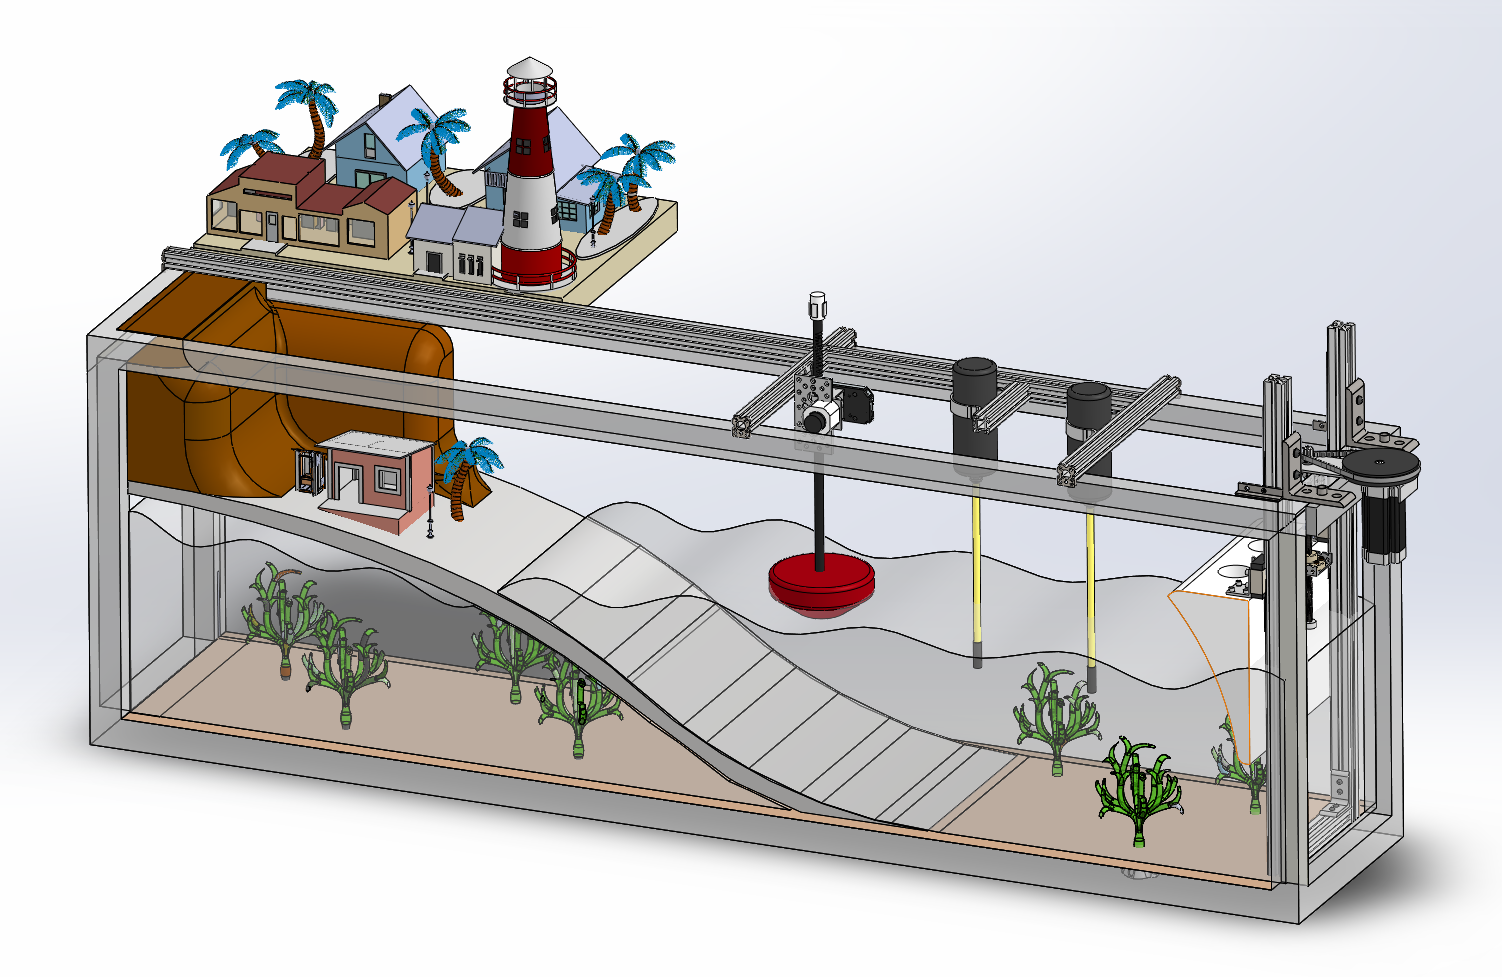
\includegraphics[width=0.75\textwidth]{diagrams/SIWEED_CAD.png}
  \caption{SIWEED CAD assembly.}
  \label{fig:CAD}
\end{figure}

\begin{figure}[tb]
  \centering
  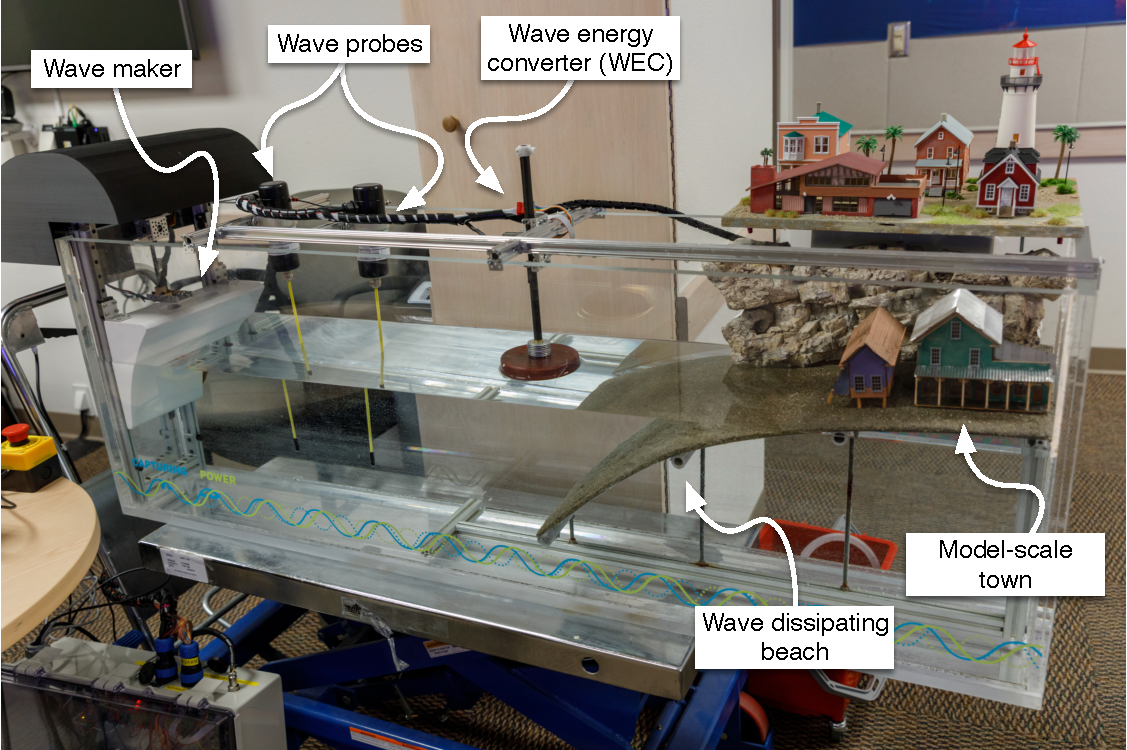
\includegraphics[width=0.75\textwidth]{diagrams/siweed_photo_with_callouts.pdf}
  \caption{Photograph of SIWEED system showing key system elements.}
  \label{fig:siweed_photo_with_callouts}
\end{figure}

\subsection{Hardware}
A system diagram for the SIWEED is shown in \figurename~\ref{fig:siweed_layout}.
Two Arduino Due micro controllers are used to control and acquire signals from the WEC and wave maker, communicating with the GUI through USB Serial.
The Windows laptop acts as the core of the system, with the two Arduino Dues attached through USB. 
Each Arduino is then attached to the various devices it communicates with.
It is worth noting that Arduino Due model was selected for their higher clock speeds, but since they operate at 3.3\,V, multiple level shifters are used to enable communication between the Arduino Dues and the components that use 5\,V logic (see\figurename~\ref{fig:siweed_layout}).

The Windows laptop runs a Processing application that acts as the GUI, data logger, and serial communication manager.
The Arduinos receive their commands from Processing over USB serial, and perform individual control loops based on control states dictated by the GUI.
One Due controls the movement of the wave maker plunger, while the other controls the torque feedback of the WEC and lights in the model town.
Each send data back to the Processing GUI for data logging and plotting purposes.
The Arduino Dues each have a number of components they communicate with through various protocols (PWM, SPI, Analog).
These perform tasks like encoder buffering, motor control, and signal generation.
The connections can be seen in \figurename~\ref{fig:siweed_layout}.

%\item \textbf{Graphical User Interface}
\subsection{Graphical User Interface}
This GUI is intended to be used with a touchscreen interface, but it is also fully functional with a mouse/track pad.
A screen shot of the GUI is shown in \figurename~\ref{fig:siweed_guiScreenShot}.
It is divided into three sections: The left instructional side, ``Mission Control", and ``System Status".

\begin{figure}[tb]
  \centering
  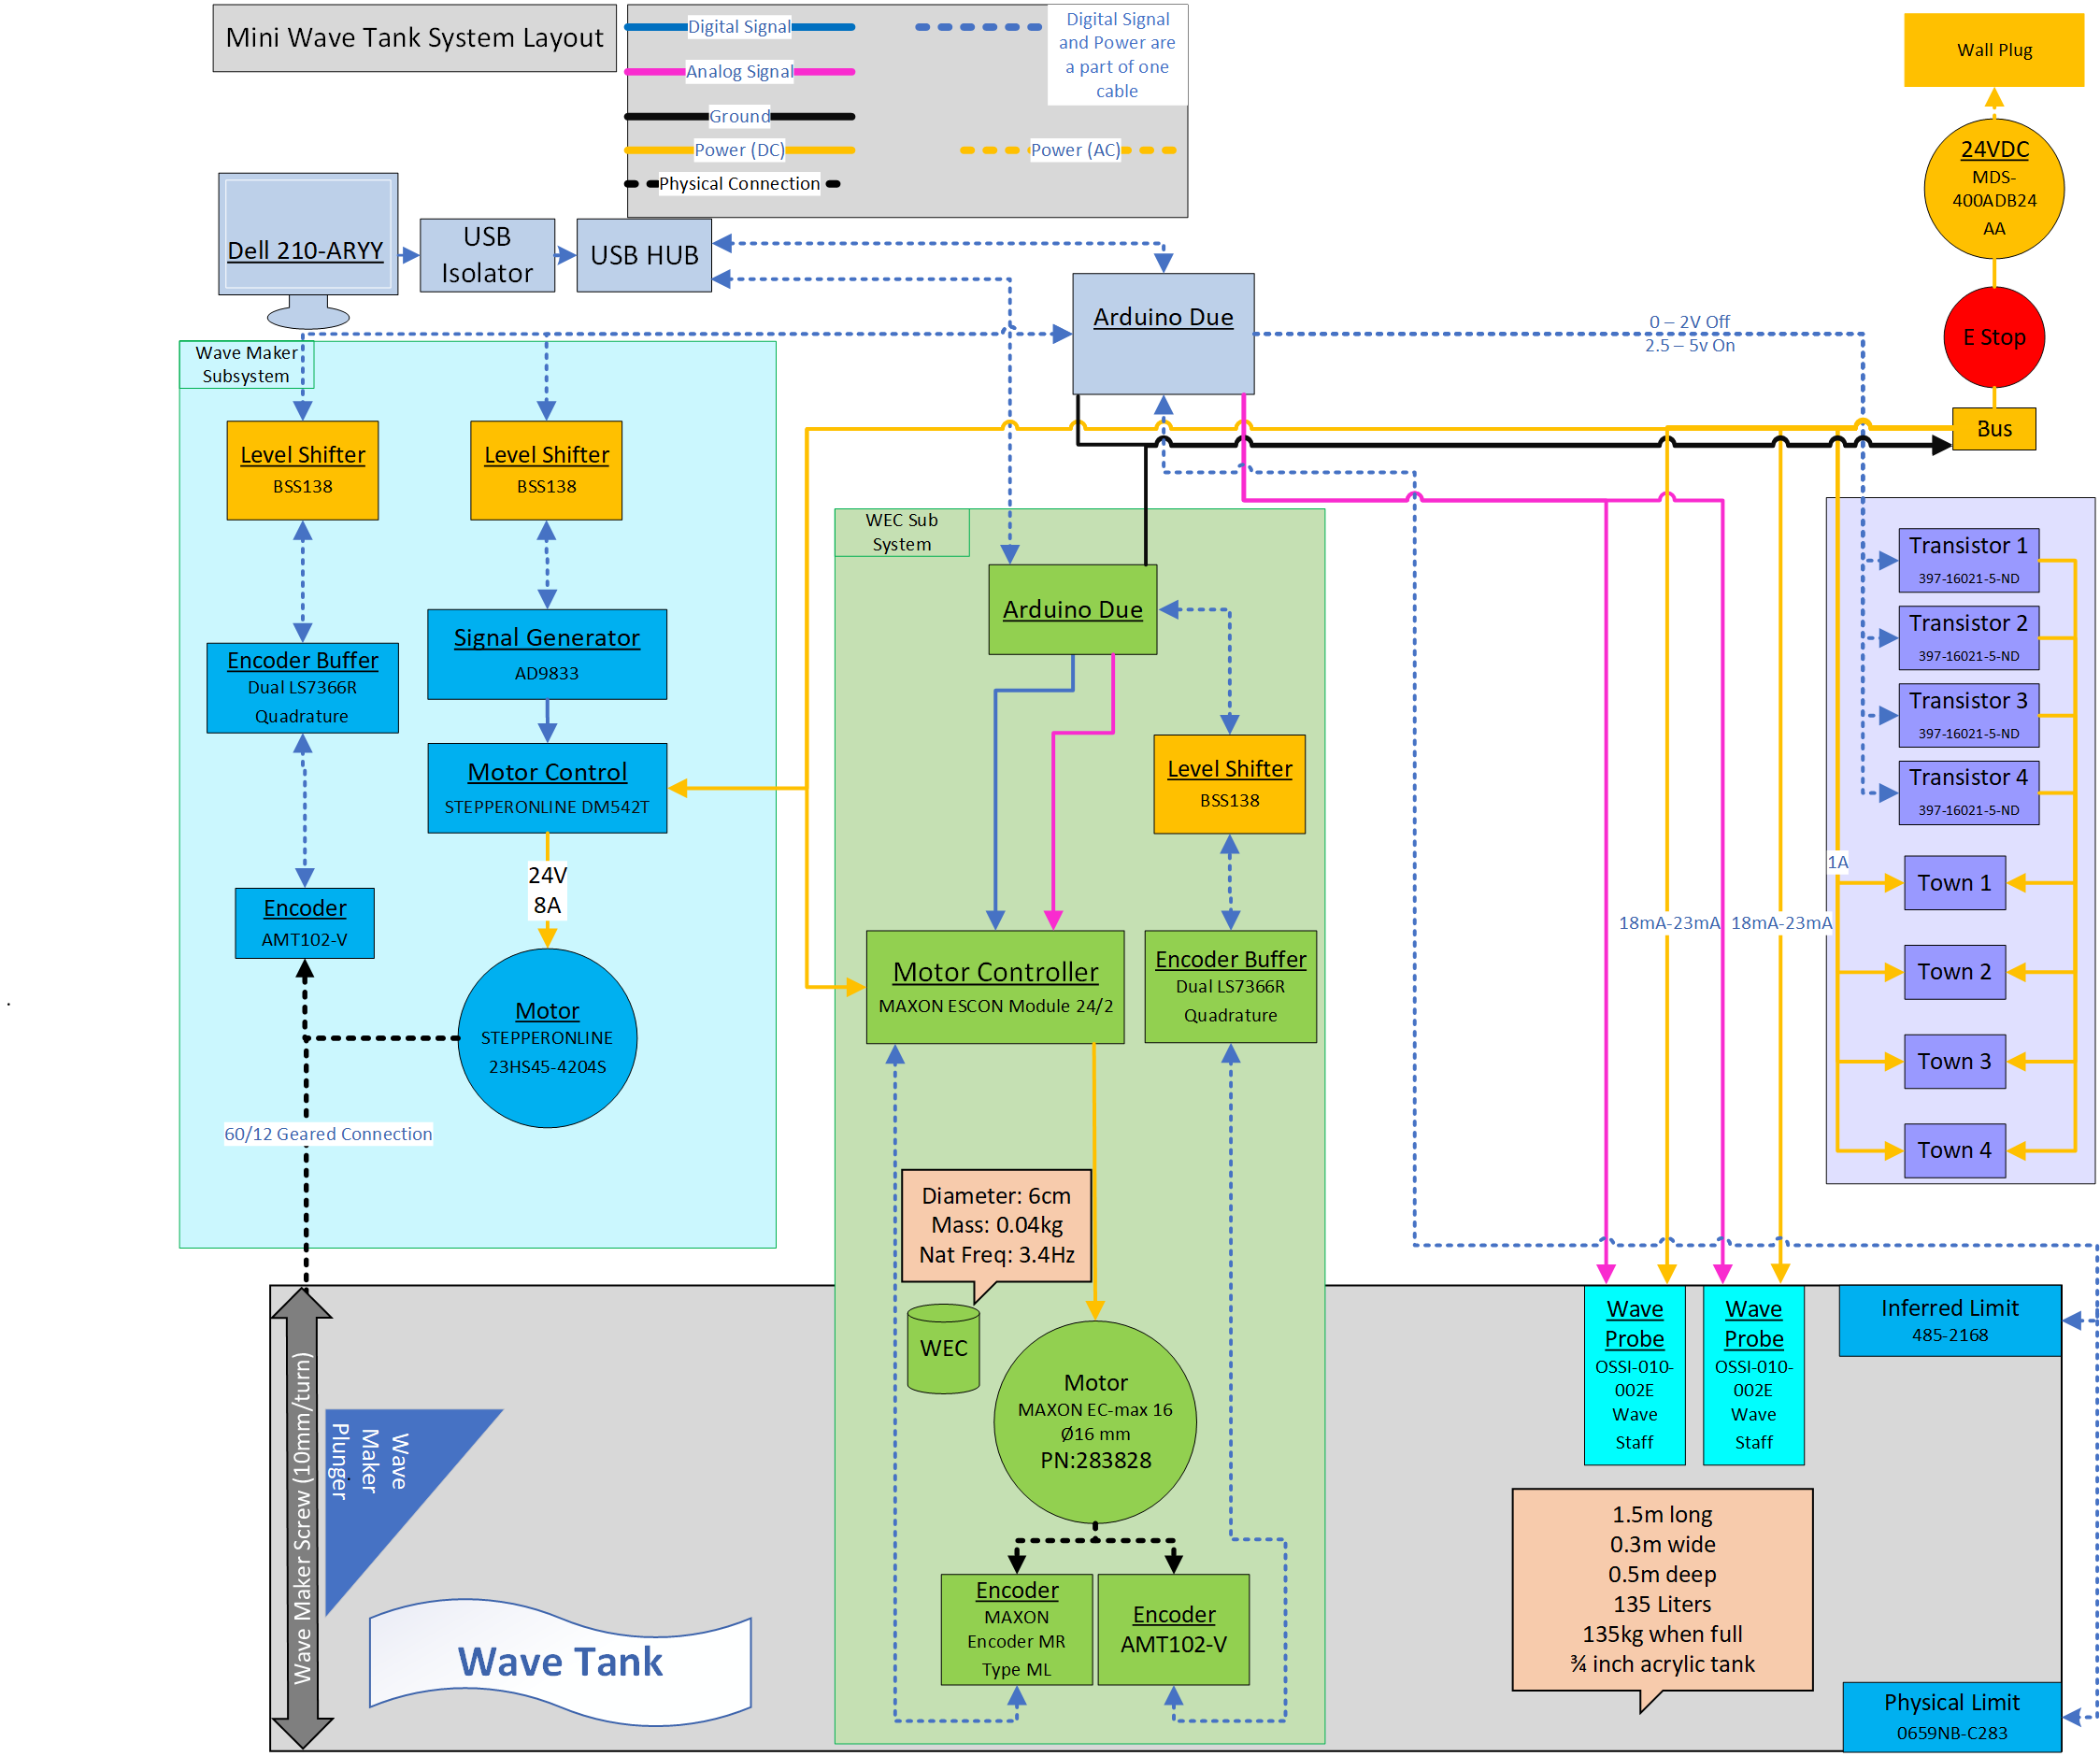
\includegraphics[width=1\textwidth]{diagrams/SystemLayout.png}
  \caption{System layout diagram.}
  \label{fig:siweed_layout}
\end{figure}
\begin{figure}[tb]
  \centering
  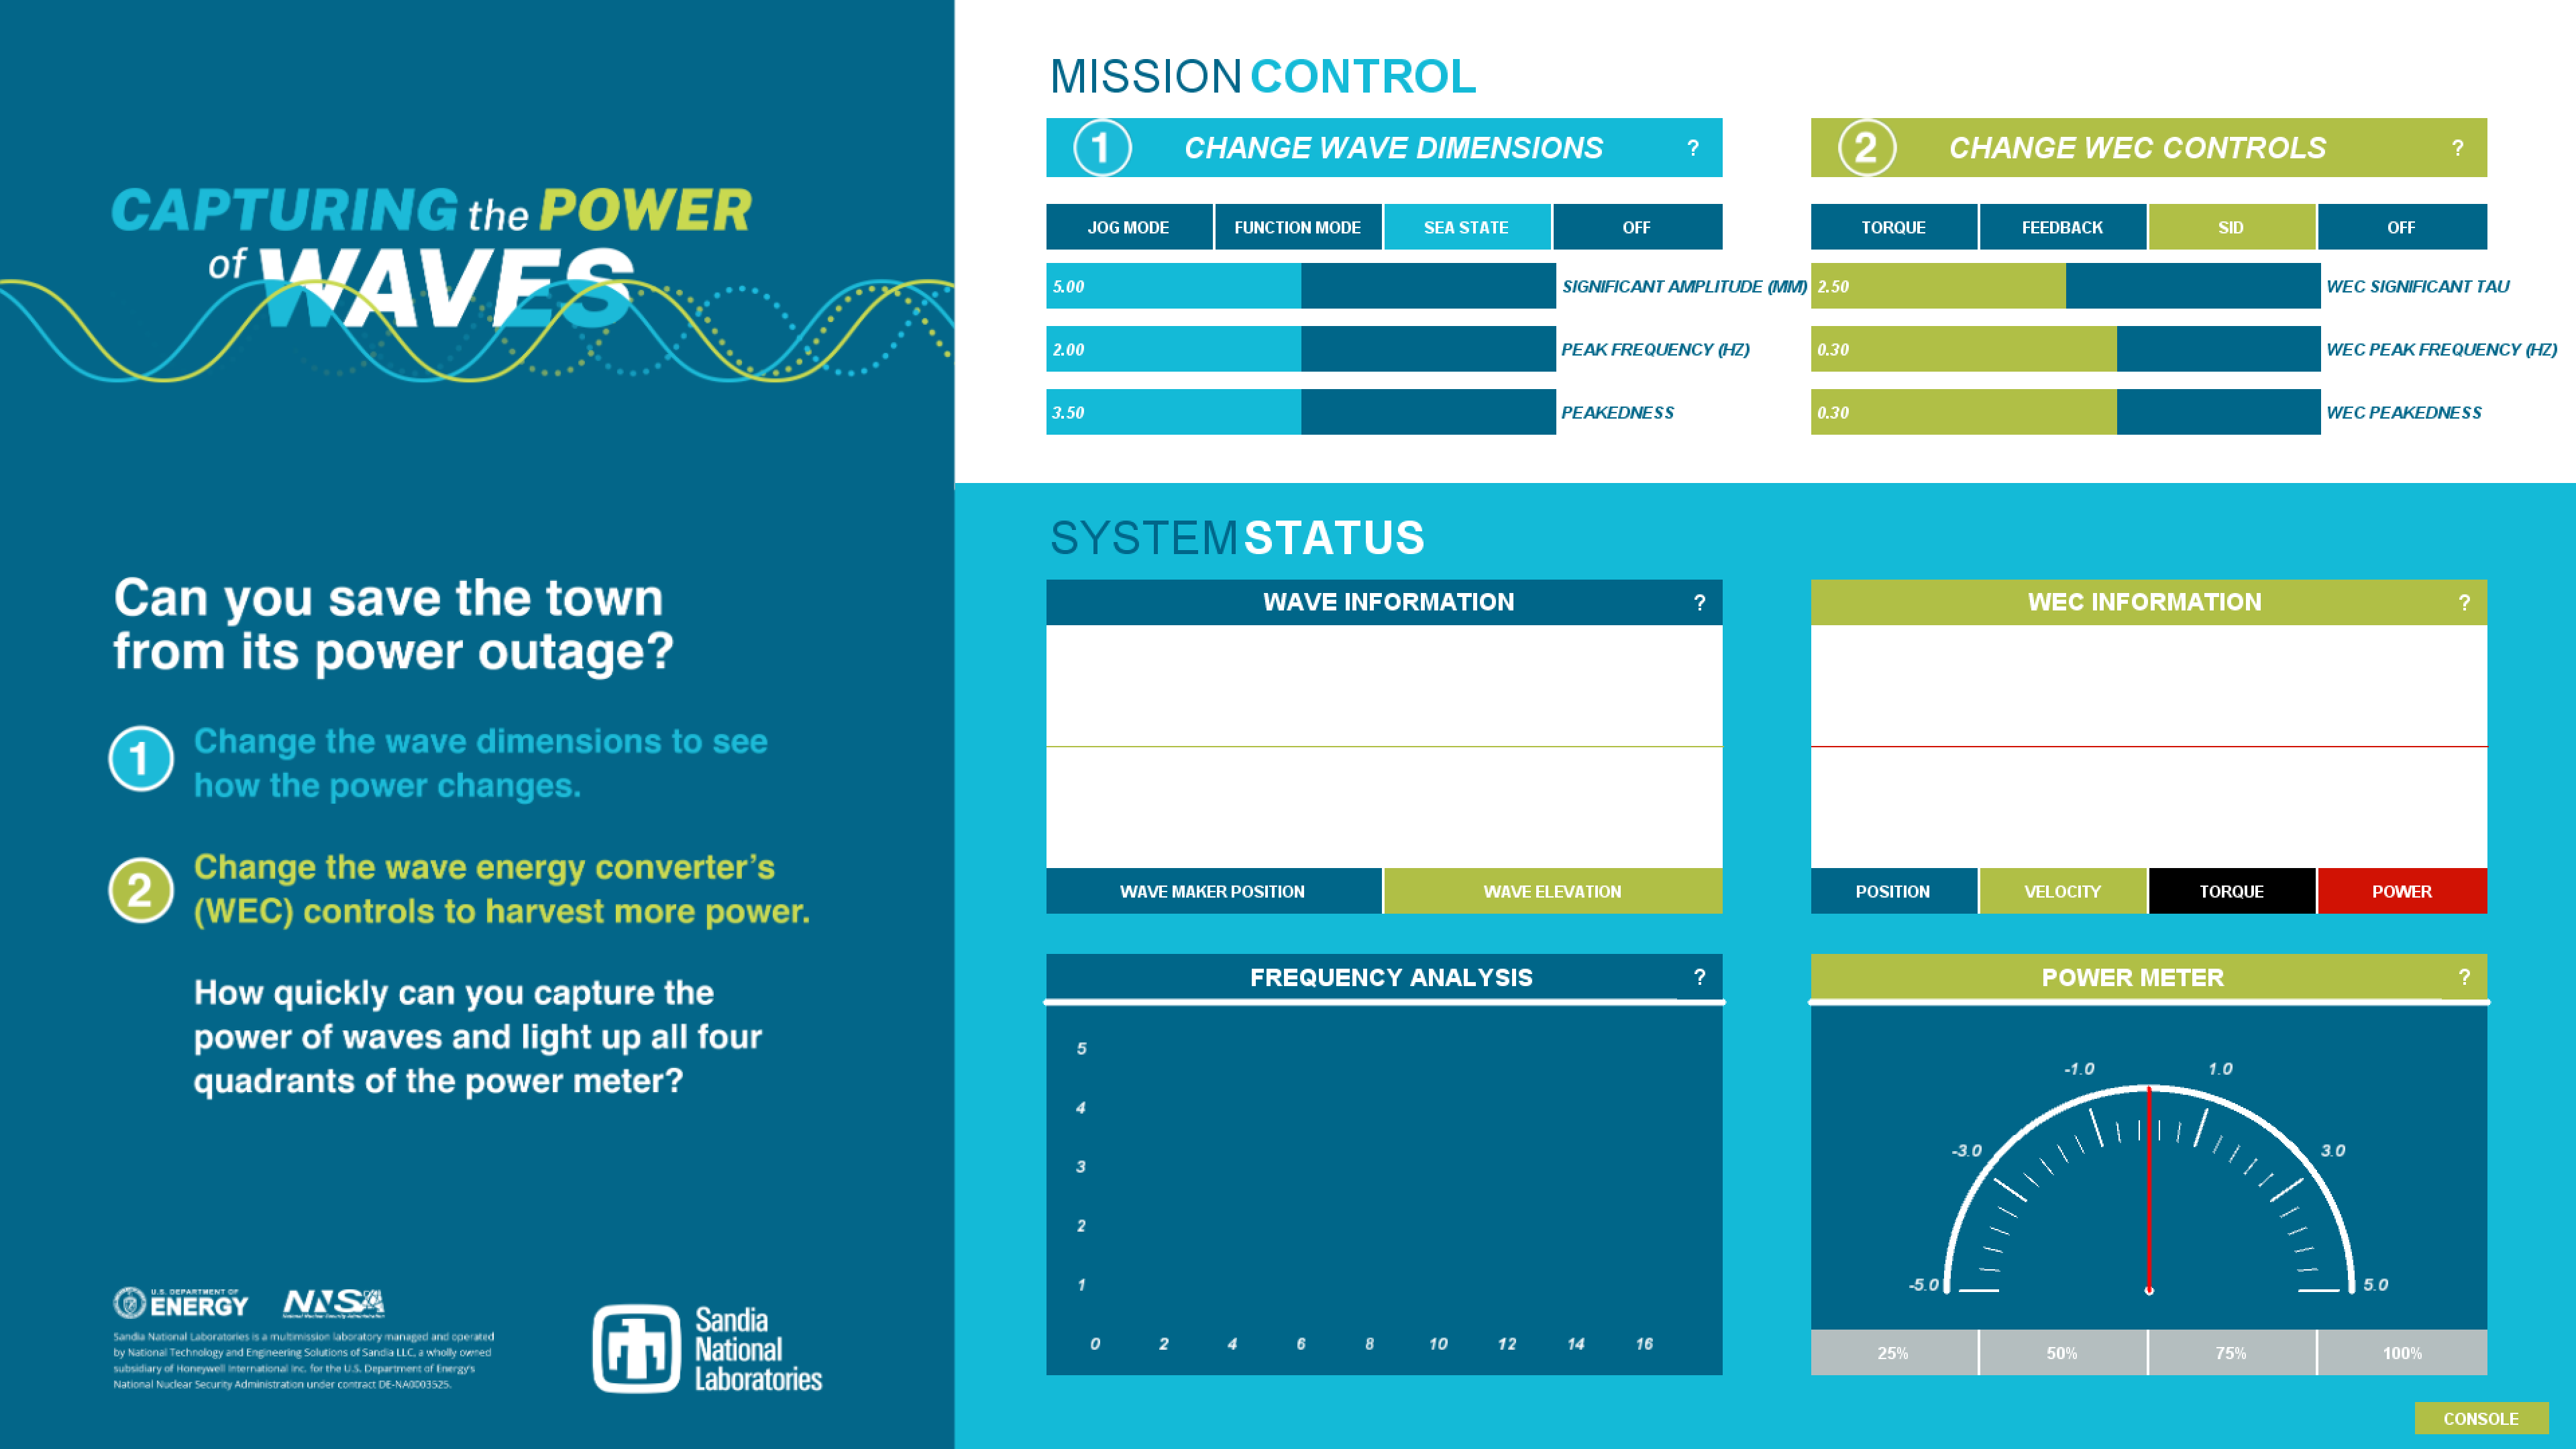
\includegraphics[width=1\textwidth]{diagrams/siweed_guiScreenShot.png}
  \caption{Graphical user interface (GUI) screenshot.}
  \label{fig:siweed_guiScreenShot}
\end{figure}

The left side of the ``Mission Control" section of the GUI pertains to control of the wave maker, which allows the user to switch between operational modes (``jog,'' ``function,'' ``sea state,'' and ``off'') and set the relevant parameters.
If, for example, the system is in ``sea state'' mode, the user can set the significant wave height ($H_s$), peak frequency ($f_p$), and peakedness factor ($\gamma$) for a JONSWAP wave spectrum.
The ``function" mode commands a simple sine wave, and so the parameters are amplitude and frequency. 
The ``jog" mode simply commands a static position for the plunger to go to, so the only input parameter is that command position.
There are only as many input sliders displayed as there are inputs to the active control mode. 
For example, if the selected mode was ``jog", only one slider would be present in that section of the GUI for the user to interact with.

The right side of the ``Mission Control" section of the GUI  contains controls for the WEC, which can be set into ``torque'' mode; in which the user directly sets a commanded torque, ``feedback'' mode; where proportional and integral feedback factors can be set by the user; ``SID'' mode, for system identification, allowing for open-loop multi-sine signals to be set by the user; and ``off.''
The ``SID'' mode works with the same inputs and JONSWAP control method as the ``Sea State'' mode for the wave maker, but commanding torque instead of position.
Where the purpose of the JONSWAP in the wave maker controls is to replicate a natural wave state, as a torque controller for the WEC, its purpose is only to provide a wide variety of torque inputs. 
This is useful when characterizing the hardware using recorded data in post-analysis (see, e.g., \cite{Bacelli2017a}).

The ``System Status" section shows two plots, one for the WEC and one for the wave maker, with each allowing the user to choose what data is plotted. 
There are multiple options for the data included in each of these plots, with the ability to plot any combination of variables simultaneously.
Each data stream is plotted in a different color, allowing the user to differentiate the various variables on each plot.
The available variables in the wave maker plot\,(left side) are ``Wave Maker Position"(as measured by the encoder) and ``Wave Elevation" (As measured from one of the submerged wave probes).
The WEC plot variables are ``Position" (measured from an encoder), ``Velocity" (differentiated from position), ``Torque" (derived from a torque constant and motor current), and ``Power" (as derived below).
Below the plots are a discrete Fourier transform of the generated waves (measured from the encoder), and a radial meter that displays the hypothetical generated power of the WEC.
That hypothetically generated power meter is driven by the same variable as the ``Power" variable in the WEC information plot above the meter, given by
\begin{equation}
  P = -\tau \cdot v .
\end{equation}
Here, $P$ is the calculated output power, $\tau$ is the torque commanded by the WEC motor controller, and $v$ is the velocity.

A number of key factors of SIWEED are:

\begin{itemize}
  \item \textbf{Open-source and documented design:} To our knowledge, the SIWEED is the first educational wave tank and WEC system to be fully documented with an open-source design and software package.
  This will enabled interested researchers and students to efficiently develop replicates and variations of the SIWEED design for their own purposes.
  \item \textbf{Portability:} To allow for transport to conferences and outreach events, the SIWEED has been specifically designed to allow for easy transportation.
  \item \textbf{WEC control:} In addition to demonstrating the physics of ocean waves, the SIWEED allows users to interact with a WEC control system to better understand the principles of reactive feedback control to maximize power absorption for the waves.
  \item \textbf{Student-led design:} The SIWEED project has been a student-led design project involving undergraduate engineering students.
  \item \textbf{Curriculum:} The SIWEED repository includes a curriculum for students K-12 based on the Next Generation Science Standards \cite{NextGenScience2021}. 
  The repository contains a presentation and a document intended to be given to the teacher beforehand. 
  The presentation explains water power and Sandia National Labs' role within the field, and then goes into more detail about wave energy converters and how the SIWEED demonstration works.
  The teacher resources document contains general information about the project, and a multitude of resources surrounding wave energy education, including videos, worksheets, vocabulary words, general topics, and Next Generation Science standards for each grade level.
\end{itemize}

\section{Design files}
%The complete design files must be either uploaded to an approved online repository, uploaded at the time of submission on the online Elsevier submission interface as supplementary materials (CAD files, videos…), or included in the body of the manuscript (e.g. figures). The two approved online repositories are Mendeley Data and the Open Science Framework (OSF instructions).
% Mendeley data: https://data.mendeley.com/
% Open Science Framework: https://osf.io/
% Open Science Framework HardwareX instructions: https://osf.io/wgk7q/wiki/home/
% > CAD files. Authors are encouraged to use free and open source software packages for creating the files. For CAD files, OpenSCAD, FreeCAD, or Blender are encouraged, but if not available source files from proprietary CAD packages such as Autocad or Solidworks and other drawing packages are acceptable.
%OpenSCAD: http://www.openscad.org/
% > 3D printing. Supplementary files that facilitate the digital replication of the devices are encouraged. For example, STL files for 3-D printing components. We recommend uploading CAD files to the NIH 3D Print Exchange as Custom Labware and providing a link to the location.
%NIH 3D Print Exchange: http://3dprint.nih.gov/
% > Electronics. PCB layouts and other electronics design files can be uploaded to the Open Hardware Repository or other repositories .
%Open Hardware Repository: http://www.ohwr.org/
% > Software and firmware. All software files used in the design and operation of the hardware should be included in the repository. Provide a description of software and firmware and use extensive comments in the code.

% Please include a summary of all design files for your hardware by filling rows of the table below

\tabulinesep=1ex
\begin{tabu} to \linewidth {|X|X|X[1.5,1]|X[1.5,1]|}
\hline
\textbf{Design filename} & \textbf{File type} & \textbf{Open source license} & \textbf{Location of the file(s)} \\\hline
%Insert design files
%\textit{Design file 1} & \textit{e.g. CAD file, figures, videos} & \textit{All designs must be submitted under an open hardware license. Enter the corresponding open source license for the file.} & \textit{Enter a link to the online location or the sentence: ``available with the article'', as appropriate}  \\\hline
Final SIWEED Town & .SLDASM & GNU GENERAL PUBLIC LICENSE & \textit{online repository} \\\hline
Hardware Hat & .SLDPRT & GNU GENERAL PUBLIC LICENSE & \textit{online repository} \\\hline
WEC\_Controller\slash interrupts.ino & .ino & GNU GENERAL PUBLIC LICENSE& \textit{online repository} \\\hline
WEC\_Controller\slash Serial.ino & .ino & GNU GENERAL PUBLIC LICENSE& \textit{online repository} \\\hline
WEC\_Controller\slash WEC\_Controller.ino & .ino & GNU GENERAL PUBLIC LICENSE& \textit{online repository} \\\hline
WaveMaker\_Controller\slash interrupts.ino & .ino & GNU GENERAL PUBLIC LICENSE& \textit{online repository} \\\hline
WaveMaker\_Controller\slash Serial.ino & .ino & GNU GENERAL PUBLIC LICENSE& \textit{online repository} \\\hline
WaveMaker\_Controller\slash WaveMaker\_Controller.ino & .ino & GNU GENERAL PUBLIC LICENSE& \textit{online repository} \\\hline
dataLogging.pde & .pde& GNU GENERAL PUBLIC LICENSE & \textit{online repository} \\\hline
Meter.pde & .pde& GNU GENERAL PUBLIC LICENSE & \textit{online repository} \\\hline
Serial.pde & .pde& GNU GENERAL PUBLIC LICENSE & \textit{online repository} \\\hline
siweedGUI.pde & .pde& GNU GENERAL PUBLIC LICENSE & \textit{online repository} \\\hline
UI.pde & .pde& GNU GENERAL PUBLIC LICENSE & \textit{online repository} \\\hline
UnitTests.pde & .pde& GNU GENERAL PUBLIC LICENSE & \textit{online repository} \\\hline
fft.java & .java& GNU GENERAL PUBLIC LICENSE & \textit{online repository} \\\hline
Complex.java & .java& GNU GENERAL PUBLIC LICENSE & \textit{online repository} \\\hline
\end{tabu}
\newline
The referenced online repository is here: \href{https://zenodo.org/record/7502670}{https://zenodo.org/record/7502670}.
\newline
% For each design file listed in the summary above, include a short description of the file below (one or two sentences)
\textbf{CAD Model:}
The CAD assembly includes all functional physical parts of the SIWEED system, with accurate dimensions that can be referenced during fabrication and assembly.
Aesthetic details, like the town are intentionally vague in the CAD model.
Physical implementation of artistic aspects are not important for functionality, but are thought to add significantly to audience engagement.
The files in the repository are Solidworks models, with all dependencies included in a compressed archive.
There is an additional part labeled ``Hardware Hat". 
This was a late addition that was 3D printed to cover potential pinch points on the model, and prevent sunlight from interfering with the infrared limit switches. 
Because it's a late addition, the part is included in the repository, but not in the final assembly. 
\par


\textbf{Processing Sketches:}
The Processing sketch is made up of multiple files combined in the processing IDE as separate tabs. 
This includes the \texttt{.pde} files and the \texttt{.java} files.
This is done mostly for organization purposes, but all files are necessary for the sketch to run properly. 
It is important to note that the sketch is also dependent on the Console library and ControlP5 library, and various graphics and text files that support the GUI. 
These files are not listed here but are all included in the online repository.
\par


\textbf{Arduino Sketches:}
Similarly to the Processing sketch, the two Arduino sketches are broken into multiple files for organization.
Once again, all files are required for the sketch to function.
It is important to note that the sketches are also dependent on various imported libraries, which are included in the online repository, but not listed here.
Some of these libraries are modified from their original versions, so it is important that they are pulled from this project repository, and not the libraries' original sources.

\section{Bill of materials}
% For a complex Bill of Materials, the complete Bill of Materials (editable spreadsheet file e.g., ODS file type or PDF file) can be uploaded in an open access online location such as the Open Science Framework repository. Include the link here. Alternatively, the Bill of Materials can be uploaded at the time of submission on the online Elsevier submission interface as supplementary material.

% > To make it easy to tell which item in the Bill of Materials corresponds to which component in your design file(s), use matching designators in both places, or otherwise explain the correspondence.

% > For material type, select from: Metal, semi-conductor, ceramic, polymer, biomaterial, organic, inorganic, composite, nanomaterial, semiconductor, non-specific, or other  
The complete Bill of Materials can be found here: \href{https://zenodo.org/record/7502670}{https://zenodo.org/record/7502670}. Note that a SIWEED system can be assembled with any tank on hand (e.g., a fish tank) and any Windows PC capable of running the Processing IDE; as these components can contribute significantly to system cost, the BOM lists the tank and computer separately from the remainder of the components.
%\textit{For a complex Bill of Materials, the complete Bill of Materials (editable spreadsheet file e.g., ODS file type or PDF file) can be uploaded in an open access online location such as the Open Science Framework repository. Include the link here. Alternatively, the Bill of Materials can be uploaded at the time of submission on the online Elsevier submission interface as supplementary material.}
%\begin{itemize}
%\item \textit{To make it easy to tell which item in the Bill of Materials corresponds to which component in your design file(s), use matching designators in both places, or otherwise explain the correspondence.}
%\item \textit{For material type, select from: Metal, semi-conductor, ceramic, polymer, biomaterial, organic, inorganic, composite, nanomaterial, semiconductor, non-specific, or other} 
%\end{itemize}
%
%\tabulinesep=1ex
%\begin{tabu} to \linewidth {|X|X|X|X|X|X|X|}
%\hline
%\textbf{Designator} & \textbf{Component} & \textbf{Number} & \textbf{Cost per unit currency} & \textbf{Total cost} & \textbf{Source of materials} & \textbf{Material type} \\\hline
%%Insert items here
%\textit{Designator} & \textit{Name of Component 1} & \textit{Number of units} & \textit{Cost per unit} & \textit{Total cost} & \textit{Source} & \textit{Material type} \\\hline
%\end{tabu}

\section{Build instructions}
%Provide detailed, step by step instructions for the construction of the reported hardware include all necessary information for reproducing the submitted hardware.
% > Explain and, when possible, characterize design decisions. Including design alternatives if they exist. 
% > Use visual instructions such as schematics, images, and videos. 
% > Clearly reference design files and component parts described in the Design File Summary and Bill of Materials. 
% >Highlight potential safety concerns that may arise

A functionally similar version of this wave tank can be reconstructed using the System Layout diagram in \figurename~\ref{fig:siweed_layout}, the bill of materials, and the CAD model shown in \figurename~\ref{fig:CAD}, which is also included in the design files.
Many parts can be substituted with similar ones, such as the laptop, transistors, power supply, or the tank itself.
Software specific hardware, such as the Arduinos or Encoder Buffers should not be substituted. 
It is important to consider safety during reconstruction: Electrical isolation and grounding, as well as guarding pinch points, is essential for safe usage.


Software setup:
\begin{enumerate}
\item Download the latest version of Arduino IDE and Processing IDE.
\item Download the Master SIWEED Repository.
\item Change the Sketchbook Location for the Arduino IDE to \texttt{\textbackslash siweed\textbackslash Arduino}.
\item Change Sketchbook Location for the Processing IDE to \texttt{\textbackslash siweed\textbackslash Processing}.
\item Change Arduino IDE board to ``Arduino Due Programming Port".
\item Upload the sketches to the Arduinos.
\item A more detailed version of these instructions can be found in the README file of the repository.
\end{enumerate}

\section{Operation instructions}
%Provide detailed instructions for the safe and proper operation of the hardware. 
%> Step-by-step operational instructions for operating the hardware. 
%> Use visual instructions as necessary. 
%> Highlight potential safety hazards.

After performing the setup described in the build instructions, the project can be operated as follows:
\begin{enumerate}
\item Power on the wavetank, ensuring any kill switches are closed, and any pinch points are clear.
\item Open processing.exe.
\item File $>$ Open $>$ \texttt{siweedGUI.pde} 
%(Ex: C\textbackslash Users\textbackslash user\textbackslash Documents\textbackslash GitHub\textbackslash siweed\textbackslash Processing\textbackslash 
%\newline siWeedGUI\textbackslash siweedGUI.pde) 
\item (optional)Edit modifiers. These are booleans at the top of the code that will do things like enable basic mode, debugging, or data logging.
\item Click ``Run".
\item The GUI will open, allow some time for it to load.
\item In the console, which will either be in the GUI, made visible by pressing the console button in the bottom right corner, or in the Processing console, depending on your boolean modifiers, unit tests should be visible that can be used to verify that everything is functioning properly. 
Note that the color of the console button in the GUI is representative of the serial checksum status.
When the received checksum matches the calculated checksum (functioning nominally), the button will be a green/yellow.
Otherwise it will be gray, indicating one of the Arduinos' checksum does not match, and the system is out of sync. 
This will result in the state of the GUI not accurately representing the state of the physical system.
\end{enumerate}

\section{Verification and characterization}
%Demonstrate the operation of the hardware and characterize its performance over relevant critical metrics
%> Demonstrate the use of the hardware for a relevant use case. 
%> If possible, characterize performance of the hardware over operational parameters. 
%> Create a bulleted list that describes the capabilities (and limitations) of the hardware. For example consider descriptions of load, operation time, spin speed, coefficient of variation, accuracy, precision and etc. 
A series of analyses were conducted on the hardware and software to confirm the proper functionality of the SIWEED.
These tests ensure that individual components, and the systems they rely on, behave as expected.
What is not included here is a series of software unit tests that run at the start of every execution of the GUI.
These test specific software functions as well as the integrity of some of the hardware and the serial communications. 
Results of these tests can be found on a per execution basis in the GUI console.
During nominal operation all unit tests have proven to pass.

\subsection{Torque constant verification:}\label{tConstSec}
The factory torque constant was verified by logging the position and current of the free floating WEC while commanding a slow sinusoidal current.
The position displacement time series was converted to a time series of the applied physical torque based on the hydrostatic force due to submerging/lifting the WEC:

\begin{equation}
  \tau = \sigma \cdot \gamma \cdot d \cdot \pi \cdot r^2
\end{equation}

\noindent{}Here, $\tau$ is torque, $\sigma$ is the radius of the pinion gear, $\gamma$ is the specific weight of water, $d$ is the displacement of the buoy in the water, and $r$ is the radius of the buoy.
%Torque = pinon radius (M)*  [9810(N/m^3)*pos(m)*pi*radius(m)^2]
It is important to note that the torque values at this point did not account for friction or hysteresis.
Plotting this torque data against the recorded commanded current values gives  \figurename~\ref{fig:TorqueConstant}.
The ``fit1'' line represents the best linear fit of the entire data set, but the data points at the highest and lowest currents are affected more significantly by static friction, so omitting them from the data set improves the torque constant estimation, as shown with the ``fit2'' line in \figurename~\ref{fig:TorqueConstant}.
This provides an estimated torque constant of about 7.52\,mNm/A, which is within 4\% of the factory stated constant of 7.8\,mNm/A.

\begin{figure}[tb]
  \centering
  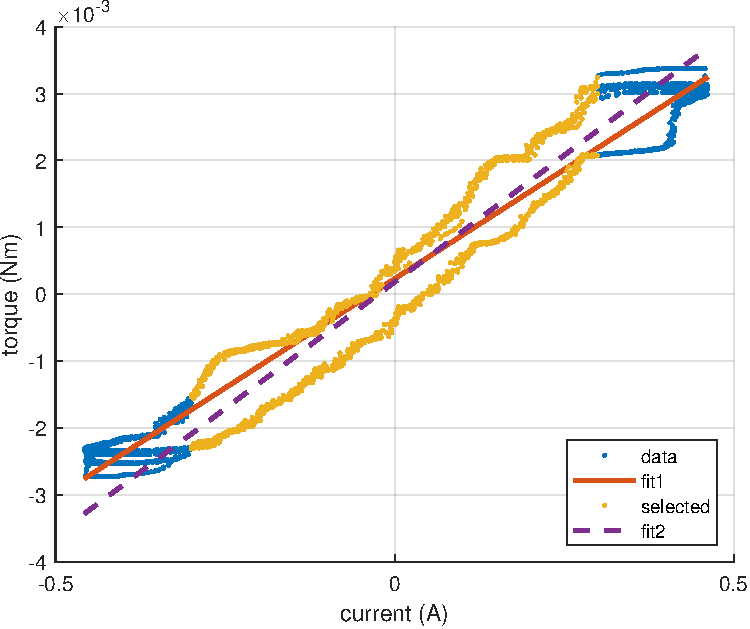
\includegraphics[width=0.75\textwidth]{diagrams/TorqueConstant.pdf}
  \caption{Torque vs commanded current, with linear fits of the entire and partial data set.}
  \label{fig:TorqueConstant}
\end{figure}


\subsection{Friction estimation:}\label{friction}
Since applied torque in Section~\ref{tConstSec} is being estimated from displacement and the frequency is low (which means that inertial and viscous effects are small), the friction shows up as a ``constant'' offset from the ideal torque constant and doesn't affect the slope.
This allows the friction to be seen as half the offset between the data points as the wave maker moves up and down moves down. 
Plotting the torque error using the calculated torque constant against the current gives \figurename~\ref{fig:TorqueError}.
The average offset shows that the static friction is about 0.45\,mNm in this operational envelope.

\begin{figure}[tb]
  \centering
  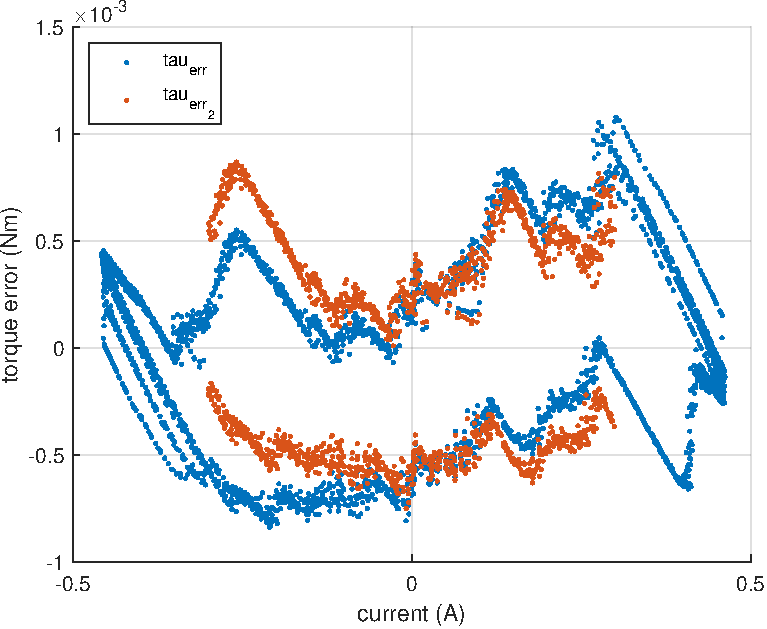
\includegraphics[width=0.75\textwidth]{diagrams/TorqueError.pdf}
  \caption{Torque error vs commanded current.}
  \label{fig:TorqueError}
\end{figure}


\subsection{Wave Probes:}	\label{waveprobes}
The readings from the wave probes could be verified by physically attaching the wave probes to the wave maker, which has a very precise encoder that allows for accurate measurement of changes in displacement.
Moving the wave maker with the wave probe attached and comparing the displacement data from both of them was used to make sure the wave probe was providing accurate readings.

It was found having two wave probes as close at they are, roughly 1\,ft apart, was problematic.
Changing the depth of one probe seemed to also adjust the reading of the nearby, stationary probe.
It is believed this is caused by capacitive coupling, but a solution was never pursued.
Known work-arounds are only using one probe, or powering the second probe off during operation.

\subsection{WEC feedback control}
The proportional derivative\,(PD) controller functions on the following formula:

\begin{equation}  \label{pdctrleq}
  \tau = k_p \cdot p + -k_d \cdot v
\end{equation}

Here, $\tau$ is the calculated torque, $k_p$ is the user defined proportional gain, $p$ is the position in meters, $k_d$ is the user defined derivative gain, and $v$ is the velocity, in meters per second, calculated by the change in position over the last 10 milliseconds. 
Using this control method allows the WEC to be controlled as a spring and damper, with the proportional gain $k_p$ adjusting the strength of the spring, and the derivative gain $k_d$ adjusting the strength of the damper.
Unlike a typical physical spring, this ``spring'' can both push device towards center, or push it away, depending on the sign of the gain.
A positive $k_p$ will act as a destabilizing force, whereas a negative $k_p$ will center the WEC to the waterline, similarly to a physical spring.

The calculation of (\ref{pdctrleq}) is done on the Arduino Due micro controller responsible for controlling the WEC, which commands an output torque through PWM to the WEC motor controller.
The position and velocity are determined with an encoder, while the $k_p$ and $k_d$ inputs are set by the user in the GUI, which the Arduino receives through USB serial.
By logging the inputs and output of the control system through a range of user inputs, its performance can be verified.
Control loop response times to be less than 33\,ms, as the data logging control loop runs at 30\,Hz and shows a delay of one sample or less.

\figurename~\ref{fig:TorqueCommanded} shows the controller during typical operation. 
The commanded torque was calculated as per (\ref{pdctrleq}), while the measured torque was taken from an analog output on the WEC motor controller that measures current, then multiplying it by the known torque constant (see Section~\ref{tConstSec}).
This shows us how the PD control algorithm and motor controller react to our given inputs.
As the linearity of the plot shows, the measured output torque closely matches the expected torque.
The standard deviation of the torque during user testing was $3.82 \times 10^{-4}$\,Nm.

\begin{figure}[tb]
  \centering
  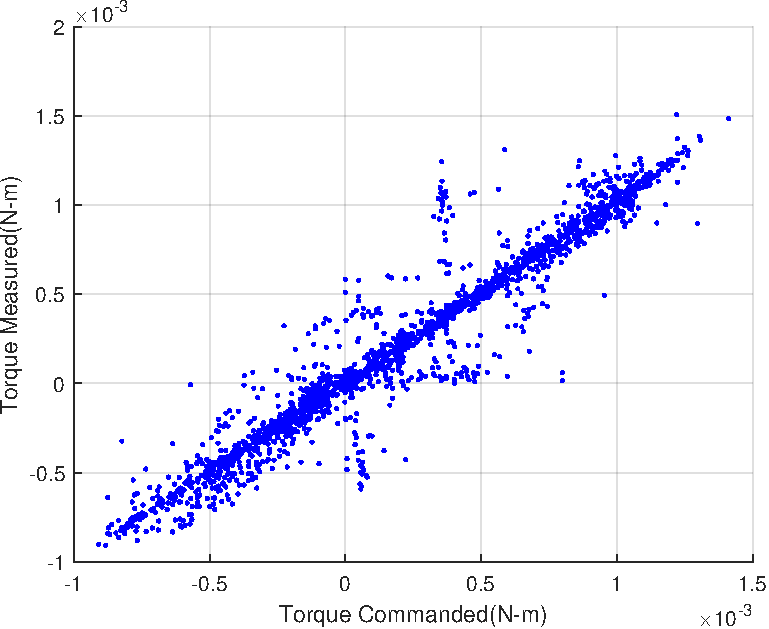
\includegraphics[width=0.75\textwidth]{diagrams/TorqueCommanded.pdf}
  \caption{Torque measured vs torque commanded.}
  \label{fig:TorqueCommanded}
\end{figure}

There is a theoretical possibility to experience saturation near the limits of our torque output.
This is the result of a protection written into the WEC motor controller, and can be adjusted by what is referred to as the ``Thermal Time Constant".
When commanded to apply a torque over what the controller deems as safe, the motor controller will apply this torque for only some time before saturating at the maximum nominal torque.
This was observed targeted testing, occurring around $3.5\times 10^{-3}$\,Nm, but not during any user tests, as the commanded torque was never that high.
If it were to become an issue, the the range of possible $k_p$ and $k_d$ commands and torque jog commands could be limited within the GUI to avoid any saturation triggers.

While fitting closely, there is still error present in this control loop. 
\figurename~\ref{fig:ErrorHistogram} shows a histogram of the torque error, calculated by subtracting the measured torque from the expected torque.
In these particular user tests, the RMS error was $9.84 \times 10^{-5}$\,Nm.
For context, the standard deviation of the torque measurement was $3.82\times 10^{-4}$\,Nm.

\begin{figure}[tb]
  \centering
  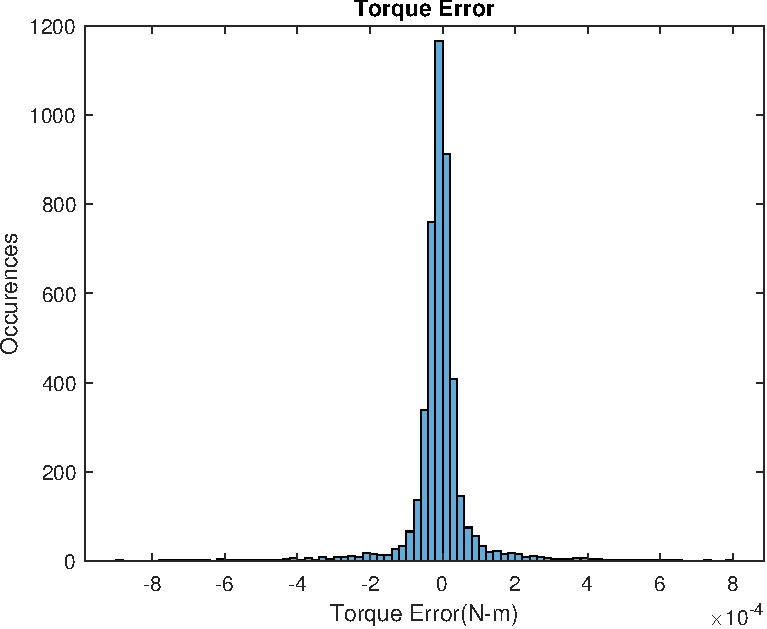
\includegraphics[width=0.75\textwidth]{diagrams/ErrorHistogram.pdf}
  \caption{Error histogram.}
  \label{fig:ErrorHistogram}
\end{figure}

Part of what has to be considered with this error is noise in the analog signal that is used to read amperage and calculate measured torque.
To characterize this, zero torque can be commanded, and then the measurement analyzed.  
For simplified data collection, user testing data sets were truncated to only sections where the commanded torque was zero.
\figurename~\ref{fig:NoiseHistogram} shows a histogram of the torque when a zero command is sent.
It can be easily seen that there is a slight positive offset in the noise, which is assumed to come from inaccuracy in the analog reporting on the motor controller, or the analog reading on the Arduino Due.
This offset varies from test to test, and can be negative.
Using this method of analyzing only data points where the torque command is zero over multiple tests gives a noise band of about $8 \times 10^{-5}$\,Nm, where 90\% of samples lie between $\pm 4 \times 10^{-5}$\,Nm.

\begin{figure}[tb]
  \centering
  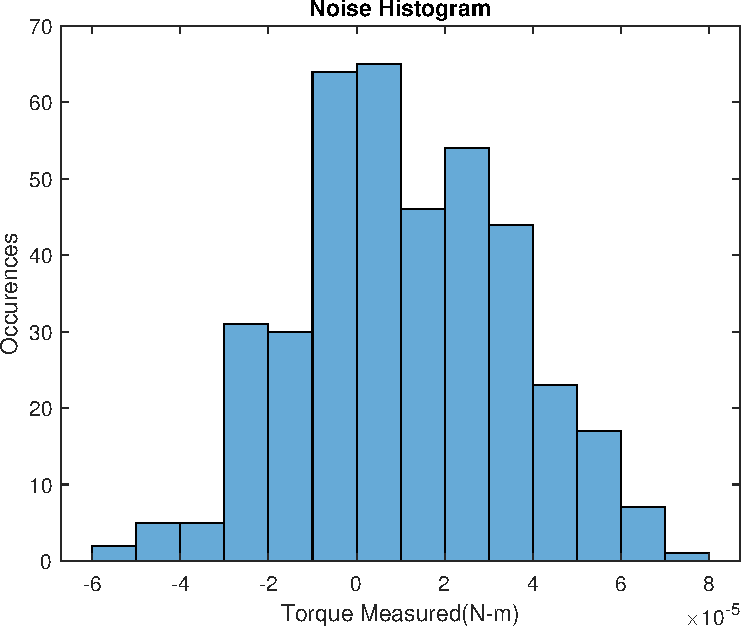
\includegraphics[width=0.75\textwidth]{diagrams/NoiseHistogram.pdf}
  \caption{Noise histogram.}
  \label{fig:NoiseHistogram}
\end{figure}


\section{Declaration of interest}
Declarations of interest: none
% a statement must be included even if there is no conflict of interest
% All authors must disclose any financial and personal relationships with other people or organizations that could inappropriately influence (bias) their work. Examples of potential conflicts of interest include employment, consultancies, stock ownership, honoraria, paid expert testimony, patent applications/registrations, and grants or other funding. Authors must disclose any interests in a summary declaration of interest statement in the manuscript file. If there are no interests to declare then please state this: 'Declarations of interest: none'. This summary statement will be ultimately published if the article is accepted. More information.}
\section{Conclusion}
The SIWEED project was developed to communicate the importance of controls within wave energy devices while adhering to the open source philosophy. 
This paper provides the resources necessary to understand and even reproduce the SIWEED, while demonstrating the viability of the system. 
With this information in hand, the owners and operators of SIWEED are now empowered to educate others about wave energy, and any interested parties are enabled to recreate this project.

Should others wish to improve the SIWEED design in future work, the wave probes module would act as an excellent start.
Because of what was believed to be capacitive coupling as described in Section~\ref{waveprobes}, and limited sensor resolution, the produced waves were never fully characterized to the user.
Communication of wave speed and a more precise wave height measurement in the GUI could prove beneficial to the user. 

\section*{Acknowledgment}
Sandia National Laboratories is a multi-mission laboratory managed and operated by National Technology and Engineering Solutions of Sandia, LLC., a wholly owned subsidiary of Honeywell International, Inc., for the U.S. Department of Energy's National Nuclear Security Administration under contract DE-NA0003525.
This paper describes objective technical results and analysis.
Any subjective views or opinions that might be expressed in the paper do not necessarily represent the views of the U.S. Department of Energy or the United States Government.

% \section{Human and animal rights}

% \textit{
% \begin{itemize}
% \item If the work involves the use of human subjects, the author should ensure that the work described has been carried out in accordance with the appropriate ethical guidelines. \item If the work involves the use of human subjects, the author should ensure that the work described has been carried out in accordance with The Code of Ethics of the World Medical Association (Declaration of Helsinki) for experiments involving humans; Uniform Requirements for manuscripts submitted to Biomedical journals. Authors should include a statement in the manuscript that informed consent was obtained for experimentation with human subjects. The privacy rights of human subjects must always be observed. \item All animal experiments should comply with the ARRIVE guidelines and should be carried out in accordance with the U.K. Animals (Scientific Procedures) Act, 1986 and associated guidelines, EU Directive 2010/63/EU for animal experiments, or the National Institutes of Health guide for the care and use of Laboratory animals (NIH Publications No. 8023, revised 1978) and the authors should clearly indicate in the manuscript that such guidelines have been followed.\end{itemize}}

% \section*{References} 
% %> Include at least one reference, to the original publication of the hardware you customized.
% %> Include other references as required. Include references to put your device in context in the literature. For more information on the reference format in HardwareX please see the Guide for Authors at: https://www.elsevier.com/journals/hardwarex/2468-0672/guide-for-authors

\bibliographystyle{plainnat}
\bibliography{refs}

\end{document}

% Author manuscript checklist 
% > HardwareX is a journal dedicated to the exhaustive and fully open source communication of advances in scientific infrastructure. Upon submission the author declares that all information necessary to reproduce the subject of the submission (e.g. bill of materials, build instructions, calibration procedures, source files, code, and safety considerations) is communicated in full and is accessible for use under an open source license.  
% > Is the subject of the submission under an open source license - as defined by the Open Source Hardware definition [http://www.oshwa.org/definition/]? 
% > Can the hardware be reproduced based on the details provided? 
% > Are all relevant design files available on the Mendeley Data or Open Science Framework server, described in the Summary of Design Files document, and clearly documented? (e.g. descriptive file names, commented code, labeled images, etc.)  
% > Do the authors use visual instructions when necessary? 
% > Do the authors describe the utility of the hardware to the scientific community? 
% > Is the performance of the hardware adequately demonstrated and characterized? 
% > Do the authors address all potential safety concerns? 

% > For more information on the article template consult the Guide to Authors [https://www.elsevier.com/journals/hardwarex/2468-0672/guide-for-authors].